\documentclass[11pt,letterpaper,twoside,openright]{report}
\usepackage[utf8]{inputenc}
\usepackage[spanish,es-tabla]{babel}

%preámbulo configuración de página
\usepackage[width=165mm,top=15mm,bottom=25mm,bindingoffset=20mm,includehead]{geometry}

%Preámbulo de Color de texto =================================================================
\usepackage{color}
\definecolor{gray97}{gray}{.97}
\definecolor{gray75}{gray}{.75}
\definecolor{gray45}{gray}{.45}
\definecolor{verde}{rgb}{0.0, 0.5, 0.0}

%preámbulo captions==========================================================================
\usepackage{caption}
\captionsetup{margin=40pt,format=hang,indention=-.5cm,font={footnotesize, rm},labelfont=bf,labelsep=colon}

%preámbulo encabezados=======================================================================
\usepackage{fancyhdr}
\pagestyle{fancy}
\fancyhead{}
\fancyfoot{}
\fancyhead[RO,LE]{\thepage}
\fancyhead[LO]{\nouppercase{\rightmark}}
\fancyhead[RE]{\nouppercase{\leftmark}}
\setlength{\headheight}{15pt} 

%preámbulo matemáticas=======================================================================
\usepackage{amsmath}
\usepackage{amsfonts}
\usepackage{amssymb}
\usepackage{dsfont}

%preámbulo sistema internacional de unidades================================================
\usepackage{siunitx}


%preámbulo referencias========================================================================
\usepackage[numbers]{natbib}
\bibliographystyle{plainnat}
\usepackage[hidelinks, breaklinks=true, backref=page,colorlinks=true,linkcolor=blue,citecolor=verde]{hyperref} 

%preámbulo de gráficos=========================================================================
\usepackage{graphicx}
\graphicspath{{figuras/}}
\usepackage{subfigure}
\usepackage{float}

%Preámbulo tabla=============================================================================
\usepackage{multirow, array}
\usepackage{booktabs}
\usepackage{colortbl}
\definecolor{SeaGreen}{rgb}{0.13, 0.7, 0.67}
\definecolor{Peach}{rgb}{0.97, 0.51, 0.47}
\definecolor{LimeGreen}{rgb}{0.31, 0.78, 0.47}
\definecolor{bananayellow}{rgb}{1.0, 0.88, 0.21}
%preámbulo de apéndices======================================================================
\usepackage[toc,page]{appendix}
\renewcommand{\appendixpagename}{Apéndices}

%preámbulo de url============================================================================
\usepackage{url}

%preámbulo de nomenclatura==================================================================
\usepackage[intoc,spanish]{nomencl}
\makenomenclature
\usepackage{etoolbox}


%Preámbulo para código de programación=======================================================
\usepackage{listings}
\lstset{ 
backgroundcolor=\color{white},
rulesepcolor=\color{black},
%
stringstyle=\ttfamily,
showstringspaces = false,
basicstyle=\footnotesize\ttfamily,
commentstyle=\color{gray45},
keywordstyle=\bfseries,
%
}
\renewcommand{\lstlistingname}{Listado}

%Preámbulo numeros decimales================================================================
\spanishdecimal{.}


%preámbulo Marcadores=======================================================================
\usepackage[hidelinks, breaklinks=true, backref=page]{hyperref} 

%Redifiniendo Titulos==========================================================================
\usepackage{titlesec}
\newcommand{\bigrule}{\titlerule[0.5mm]}
\titleformat{\chapter}[display] % Se cambia el formato del capitulo
%{\bfseries\Huge} % por defecto se usarán caracteres de tamaño \Huge en negrita
{\bfseries\Huge} % por defecto se usarán caracteres de tamaño \Huge en negrita
{% contenido de la etiqueta
\titlerule % línea horizontal
\filright % texto alineado a la derecha
\Large\chaptertitlename\ % "Capítulo" o "Apéndice" en tamaño \Large en lugar de \Huge
\Large\thechapter} % número de capítulo en tamaño \Large
{0mm} % espacio mínimo entre etiqueta y cuerpo
{\filright} % texto del cuerpo alineado a la derecha
[\vspace{0.5mm} \bigrule] % después del cuerpo, dejar espacio vertical y trazar línea horizontal gruesa

%Preámbulo utilidades=========================================================================
\usepackage{pdfpages}	%Incluye hojas de de archivos PDF
\usepackage{siunitx}			%Sitema internacional de unidades
\usepackage[T1]{fontenc}	%Fuentes
\usepackage{textcomp}		%Fuentes

%preámbulo teoremas, Definiciones y Proposiciones ==============================================================================================================
\newtheorem{teo}{Teorema}[chapter]
\newtheorem{ejem}{Definición}[chapter]
\newtheorem{prop}{Proposición}[chapter]
\newtheorem{obs}{Observación}[chapter]
\newtheorem{lema}{Lema}[chapter]

%preámbulo acronimo ===================================================
\usepackage{acronym}
\acrodef{fl}[FL]{Función de Lyapunov} \acused{fl}
\acrodef{pd}[p.d.]{positiva definida}
\acrodef{ae}[AE]{asintóticamente estable}
\acrodef{gae}[GAE]{global y asintóticamente estable}


%preámbulo de nomenclatura ==========================================
\usepackage[intoc, spanish]{nomencl}
\makenomenclature
\nomenclature{$MCC$}{Modo de conducción continua}
%FIN DEL PREÁMBULO===================================================

%====================================================================
%====================================================================
%                    INICIO DEL DOCUMENTO
%====================================================================
%====================================================================

\begin{document}
	\chapter{Introducción}
	Generalmente en los sistemas de control no todos los estados están disponibles para su medición, por ello  es necesario diseñar observadores o estimadores para poder conocerlos. La tarea básica de un observador es estimar variables no medidas a partir de las mediciones y el conocimiento del modelo, esto es posible solo si hay suficiente información disponible, \textit{i.e.} si el sistema es observable (o detectable). \vspace{.3cm}
	
	En la actualidad el problema de diseño de observadores para sistemas lineales a sido ampliamente estudiado y existen diferentes métodos de diseño. Todo lo contrario con respecto al diseño de observadores para sistemas no lineales \cite{Besancon2007}.  \vspace{.3cm}

	El diseño de Observadores parea sistemas no lineales  ha sido estudiado por medio de la teoría de disipatividad, dicha técnica ha demostrado ser eficiente para ciertas clases de sistemas no lineales. \vspace{.3cm}
	
	La disipatividad fue desarrollada en los 60's y 70's especialmente por J. C. Willeams \cite{Willems1972PartI}, \cite{Willems1972PartII}, para entender las propiedades de estabilidad de los sistemas interconectados. La teoría de disipatividad ha sido motivada por los trabajos sobre el problema de estabilidad absoluta, el criterio de Popov, el trabajo de Yakubovich, el lema Kalman-Yakubovichc
	 y la pasividad.\vspace{.3cm}
	
	 La idea de utilizar conceptos de disipatividad para el diseño de observadores se ha utilizado en \cite{Moreno2001}, \cite{Shim2003}, \cite{Moreno2004}, \cite{Moreno2005}, \cite{Rochacozatl2004},\cite{Rochacozatl2011}, en los cuales se usa la teoría de disipatividad para contrarrestar los efectos de las no linealidades en el diseño de observadores lineales. Además, la clase de sistemas que son disipativos por naturaleza puede ser ampliada para otros sistemas mediante una retroalimentación del estado o de la salida, como ha se a mostrado en \cite{Byrnes1991} y \cite{Rocha2001}.  \vspace{.3cm}
	 
	 
	Los observadores con entradas desconocidas son una clase especial de estimadores que son capaces de reconstruir el estado de un sistema, a pesar de las entradas inciertas. El diseño de estos observadores puede ser basándose en un diseño disipativo o en un diseño por modos deslizantes.\vspace{.3cm}
	
	En el caso de los sistemas lineales  invariantes en el tiempo (LTI) con entradas desconocidas, la detectabilidad fuerte* (detectabilidad fuerte y grado relativo uno) es una condición necesaria y suficiente para asegurar la existencia de un observador \cite{Hautus1983}. El problema de existencia de un OUI para el sistema LTI con entradas desconocidas arbitrarias, ha sido analizado bajo un enfoque de disipatividad \cite{Moreno2001}, donde la existencia de un observador es equivalente a la posibilidad de hacer que la planta sea disipativa por inyección de salida (ver Figura \ref{Fig: Capitulo1 - Condiciones de existencia para un UIO}).
	
	\begin{figure}[hbtp]
		\centering
		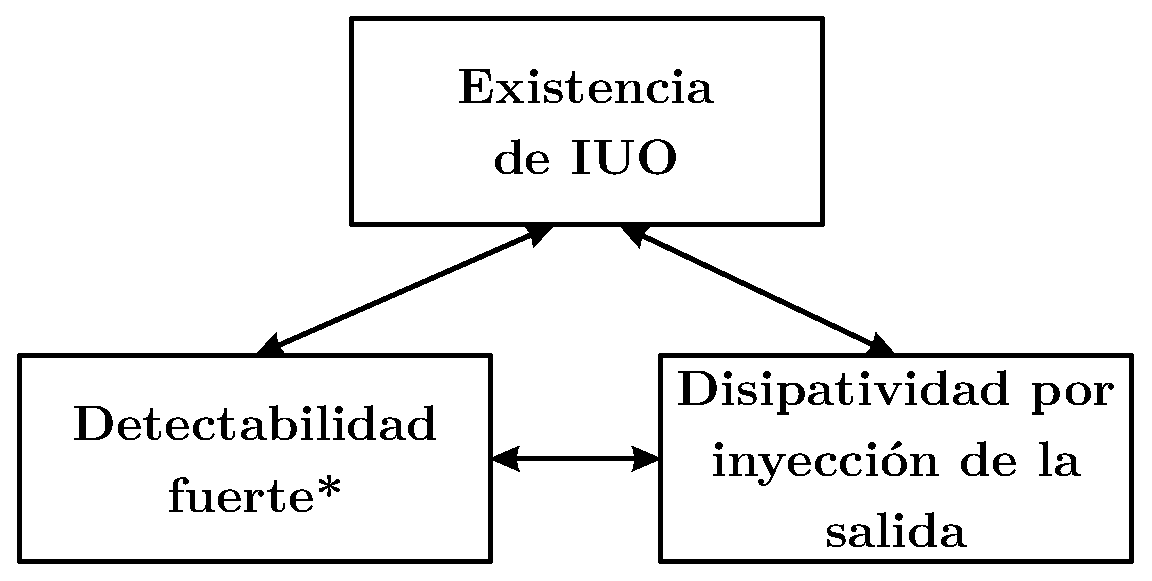
\includegraphics[width=8cm]{Capitulo1_CondicionDeExistenciadeUIO.eps}
		\caption{Condiciones de existencia para un UIO.}
		\label{Fig: Capitulo1 - Condiciones de existencia para un UIO}
	\end{figure}
	\newpage
	En sistemas no lineales con entradas desconocidas, las condiciones para la existencia de un UIO no están muy bien establecidas, como es el caso de los sistemas LTI. Un análisis similar al caso de los sistemas lineales presentado en \cite{Moreno2001}, resultó en una propiedad disipativa incremental para los sistemas no lineales MIMO con entradas desconocidas, donde existe la posibilidad de hacer a la planta disipativa mediante una inyección de la salida, satisfaciendo la condición de grado relativo uno, la cual es necesaria para la existencia de un observador con entradas desconocidas (\cite{Rochacozatl2004}). El enfoque disipativo también es aplicable a sistemas con no linealidades discontinuas o multivaluadas como se mostró en  \cite{Osorio2006} y \cite{Baltazar2010}. 
	
	Una interpretación dinámica de los conceptos de observabilidad fuerte y detectabilidad para sistemas no lineales con perturbaciones inciertas fue hecha en \cite{Moreno2014}, lo que permite tratar el problema de la existencia del observador para sistemas no lineales.
	
	El grado relativo uno es una condición necesaria para la existencia de un observador con entradas desconocidas en sistemas lineales y no lineales con perturbaciones inciertas arbitrarias. Esto representa una restricción para la clase de sistemas que se pueden tratar, ya que la presencia de perturbaciones inciertas con un grado relativo mayor que uno se da en muchos sistemas, e.g. sistemas mecánicos y sistemas electromecánicos. Cuando el grado relativo es mayor que uno, es necesario conocer características de la perturbación incierta (por ejemplo su cota), para diseñar el observador.
	
	Si la perturbación incierta es acotada, los observadores disipativos pueden proporcionar la convergencia del error de estimación a una región cercana al origen.
	
	En los sistemas LTI con entradas desconocidas acotadas y bajo la condición de detectabilidad/observabilidad fuerte (ausencia de zeros invariantes), el diseño de observadores por modos deslizantes (SMO), para sistemas de grado relativo uno con respecto a la entrada desconocida, fue estudiado en \cite{WalcottZak}.
	
	Cuando el grado relativo de la entrada desconocida con respecto a la salida es más grande que uno, la diferenciación de la salida es necesaria. Sin embargo, un inconveniente de los observadores por modos deslizantes y su proceso de diferenciación, es que la mayoría de ellos, necesita que el vector de  estado afectado por la entrada desconocida esté delimitado de manera uniforme, en este caso se requiere la propiedad BIBS. 
	
	El primer diferenciador por modos deslizantes que aparece en la literatura, es el basado en el Algoritmo Super-Twisting (STA) (\cite{Levant1998}). Este diferenciador por modos deslizantes se define como 
	\begin{eqnarray}
	\dot{z}_1&=&-1.5L^{\frac{1}{2}}|z_1 -f(t)|^{\frac{1}{2}}sign(z_1 -f(t))+z_2\\
	\nonumber \dot{z}_2&=&-1.1L\; sign(z_1 -f(t))
	\end{eqnarray}
	el cual  garantiza una estimación en tiempo finito, de la derivada del tiempo de f(t) cuando $|\dot{f}(t)|\leq L$, donde $z_1-f(t)$ y $z_2-\dot{f}(t)$ son llevados a cero en tiempo finito. El uso del diferenciador de Levant se encuentra ampliamente reportado \textit{i.e.} \cite{Davila2005},\cite{Davila2006}, \cite{Bejarano2007}.
	\newpage
	Para superar la necesidad de la propiedad BIBS en los  sistemas LTI con  entradas desconocidas en el diseño de UIO, en el trabajo de \cite{Fridman2007} se propone la conexión en cascada de dos observadores (ver Figura \ref{Fig: Capitulo1 - Observador en cascada LTI}); un observador de Luenberger, el cual lleva al error de estimación a una región cerca de origen, y un diferenciador por modos deslizantes de orden superior (HOSM), el cual permite una estimación teóricamente global y en tiempo finito a los estados del sistema. 
	
	\begin{figure}[hbtp]
	\centering
	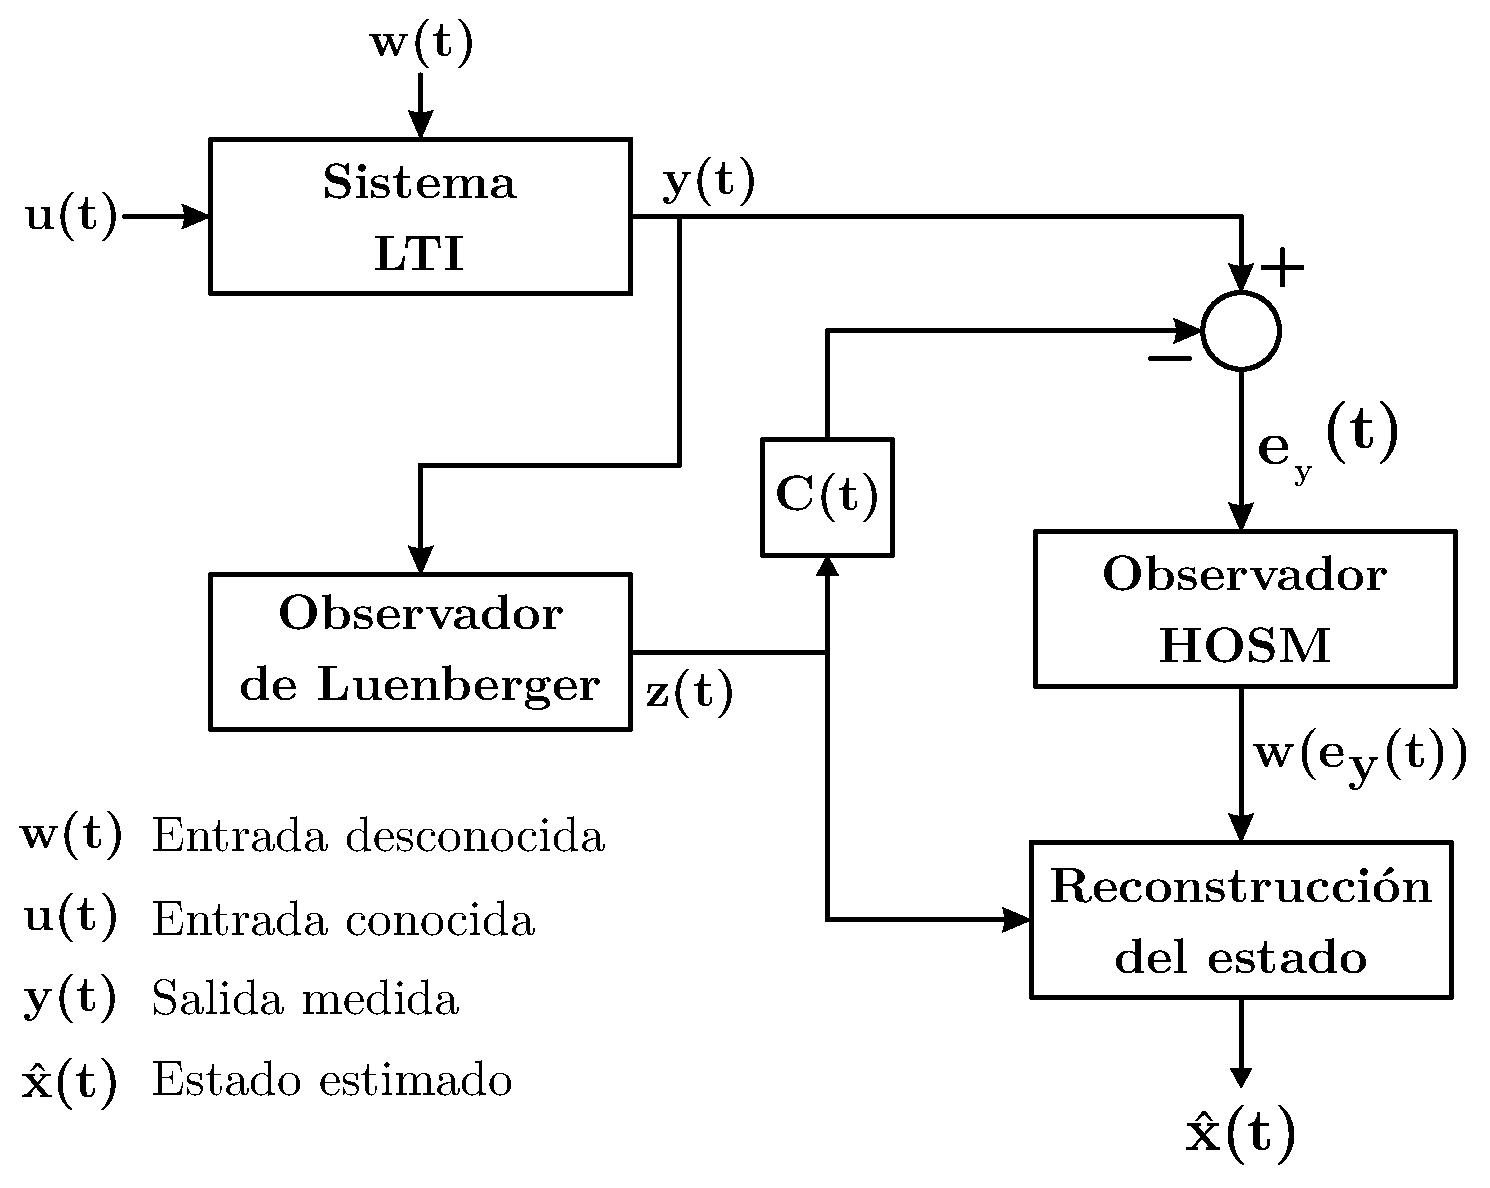
\includegraphics[width=10cm]{Capitulo1_CascadaLTI.eps}
	\caption{Observador en cascada.}
	\label{Fig: Capitulo1 - Observador en cascada LTI}
	\end{figure}	 

	Para el caso de sistemas no lineales, en \cite{Apaza2018Higher}  se propone un observador por modos deslizantes de orden superior con estabilizadores disipativos escalados (ver Figura \ref{Fig: Capitulo1 - Observador en cascada NLTI}); en dicho trabajo se muestra y  se prueba que la conexión en cascada directa, de un observador disipativo con un diferenciador HOSM proporciona una estimación teóricamente exacta en tiempo finito de los estados reales. Dicha conexión directa presenta algunos inconvenientes debido a que las ganancias del diferenciador HOSM crecen junto con las ganancias disipativas del observador. Es por tal motivo, que en el mismo trabajo se propone un Estabilizador Disipativo a Escala (EDE). Este EDE garantiza que las ganancias del diferenciador HOSM se puedan elegir, de acuerdo con el límite superior de la entrada desconocida. Además, las ganancias del estabilizador disipativo escalado pueden crecer y no afectar las ganancias del diferenciador HOSM. En consecuencia, se puede lograr la convergencia exacta en el tiempo finito global del observador de diferenciador HOSM disipativo escalado en cascada.
	\begin{figure}[hbtp]
	\centering
	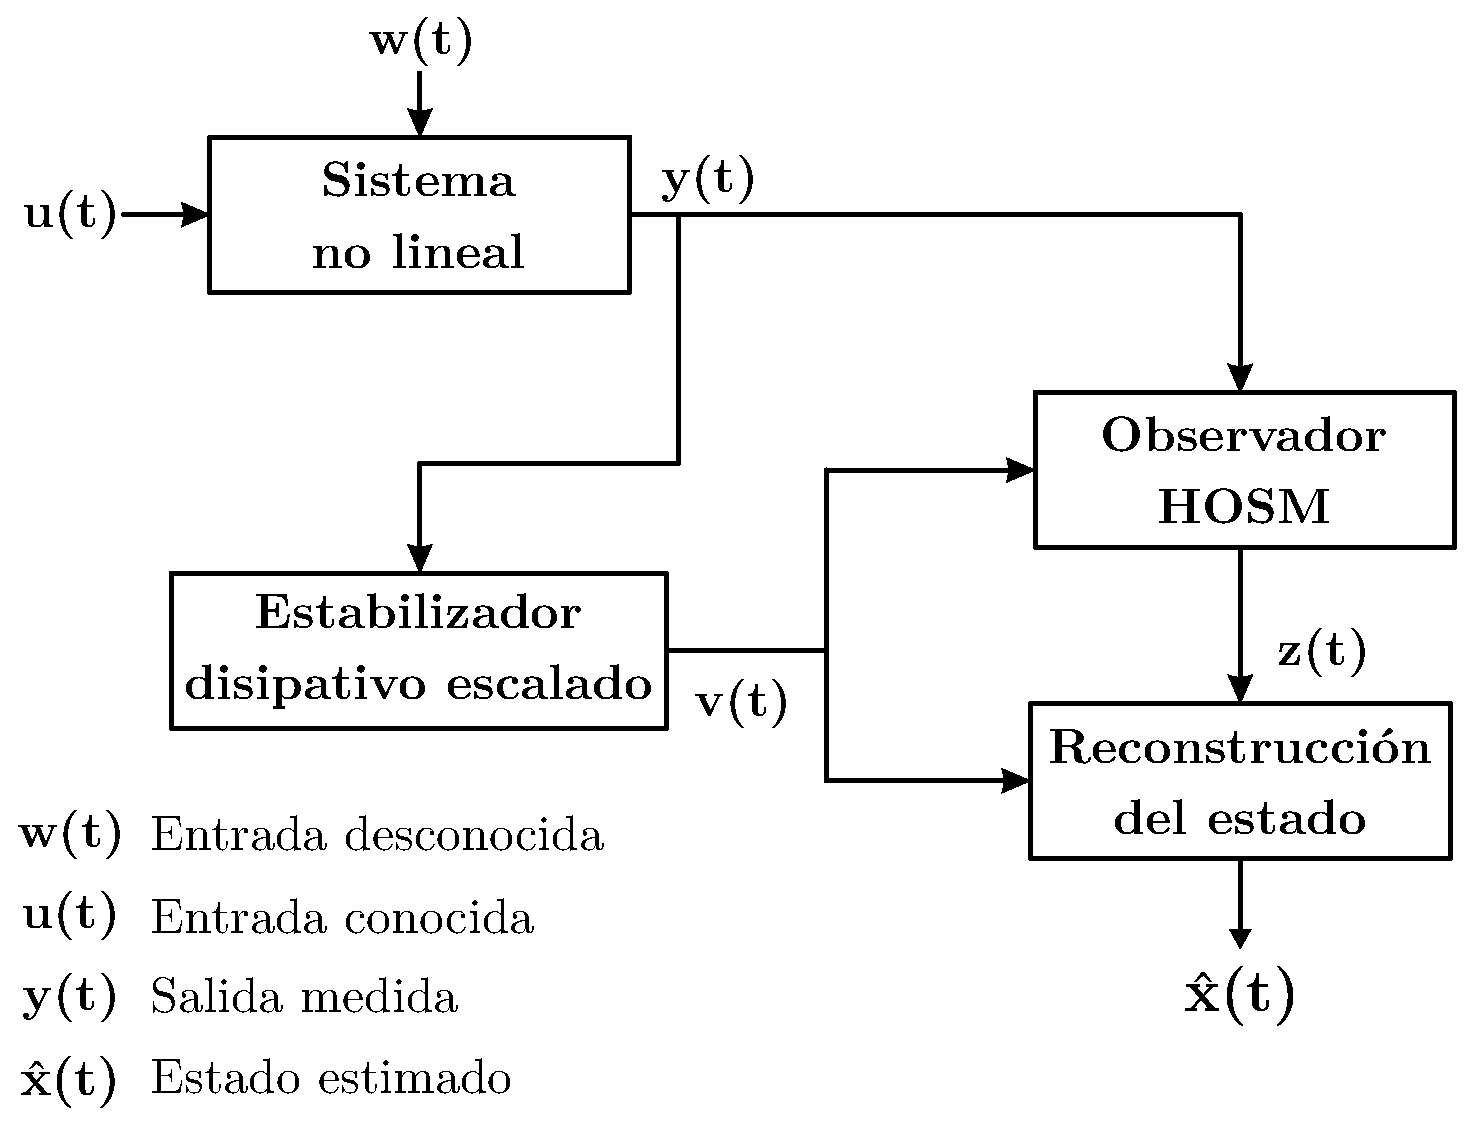
\includegraphics[width=10cm]{Capitulo1_CascadaNLTI.eps}
	\caption{HOSM y observadores disipativos bajo un esquema en cascada.}
	\label{Fig: Capitulo1 - Observador en cascada NLTI}
	\end{figure}
 	 La principal desventaja de los dos métodos mencionados tanto para sistemas lineales como no lineales es que el orden de los observadores es dos veces el orden del sistema, además del difícil calculo de las ganancias.
	
	Un observador del mismo orden del sistema, que combina propiedades disipativas con modos deslizantes fue propuesto en \cite{Apaza2018Dissipative}, la idea consiste en construir un observador que estabilice el error de observación con ayuda de propiedades disipativas, y que asegure la convergencia del error de estimación de manera exacta y en tiempo finito mediante modos deslizantes. En dicho trabajo, la dinámica del error de observación es localmente homogénea. Por lo tanto, en torno al origen, el observador tiene las  mismas propiedades que el diferenciador de Levant \cite{Levant1998}. Sin embargo, éste enfoque fue desarrollado para sistemas mecánicos con grado relativo dos, y en la actualidad no existe una metodología para extender este resultado a sistemas con grado relativo mayor a dos. Además, el diseño de las ganancias es complejo.
	
		En resumen, los observadores en cascada y escalados, presentan un difícil diseño de ganancias  y  los observadores disipativos y los observadores por modos deslizantes requieren 
	condiciones restrictivas para su buen desempeño en presencia de UP: la condición BIBS para los observadores por modos deslizantes y grado relativo uno para los  observadores disipativos (ver Tabla \ref{Tab: Capitulo1 - Características de los observadores}).
	
	\begin{table}[H]
		\caption{Características de los observadores por modos deslizantes y los basados en disipatividad. }
		\resizebox{16cm}{!} {
			\begin{tabular}{c|c|c|c|c|c}
				\toprule
				\cellcolor{SeaGreen} \textbf{Observador} &\cellcolor{SeaGreen} \textbf{UP} &\cellcolor{SeaGreen}  \textbf{Grado relativo}&\cellcolor{SeaGreen} \textbf{Propiedad BIBS}  &\cellcolor{SeaGreen} \textbf{Estimación} &\cellcolor{SeaGreen} \textbf{Tipo de observador}\\\toprule
				\cellcolor{SeaGreen} Disipativo&Arbitraria  &\cellcolor{Peach}  uno  &\cellcolor{LimeGreen} no requiere  &\cellcolor{LimeGreen}  asintotica &\cellcolor{LimeGreen} global  \\\midrule
				\cellcolor{SeaGreen} Modos deslizantes &acotada &\cellcolor{LimeGreen} más grande que uno  &\cellcolor{Peach}   requiere &\cellcolor{LimeGreen} en tiempo finito  &\cellcolor{Peach}    local\\\toprule
		\end{tabular}}
		\label{Tab: Capitulo1 - Características de los observadores}
	\end{table}

	\section{Planteamiento del problema}
	Se aborda el problema del diseño de observadores con entradas desconocidas  para sistemas no lineales que no poseen  la propiedad BIBS. En este sentido, se consideran las siguientes clases de sistemas no lineales.
	\subsection{Primera clase de sistemas no lineales}
	Considere el sistema de segundo orden no lineal con entradas desconocidas 
	\begin{equation}
	\label{Ecu: Capitulo1 - Primera clase de sistemas}
	\begin{split}
	\dot{x}_1&=x_2+\psi(x_1,x_2),\\
	\dot{x}_1&=u-w(t),\\
	y&=x_1
	\end{split}
	\end{equation}
	donde $x_1,\;x_2 \in \mathbb{R}$ son los estados, $y$  la salida medida , $u$  la entrada conocida, $w(t)$ la entrada desconocida y $\psi$ es una  no linealidad del sistema.
	
	Para \eqref{Ecu: Capitulo1 - Primera clase de sistemas} considere el siguiente observador de estados,
	\begin{eqnarray}
	\label{Ecu: Capitulo1 - Oservador 1}
	\nonumber \dot{\hat{x}}_1&=&\hat{x}_2+\psi (y,x_2+(\hat{x}_2-x_2)+k_3\phi_3)-k_1\phi_1,\\
	\dot{\hat{x}}_2&=&-k_2\phi_2+u,
	\end{eqnarray}
	donde $\hat{x}_1$, $\hat{x}_2$ son lo estados estimados del sistema, $k_1$, $k_2$, $k_3$ son ganancias de diseño y $\phi_1$, $\phi_2$, $\phi_3$  representa  términos de corrección. 
	
	El objetivo es diseñar a los términos de corrección de tal manera que  \eqref{Ecu: Capitulo1 - Oservador 1} sea homogéneo y que sus estados  converjan  de forma  global, exacta y en tiempo finito a los estados del sistema \eqref{Ecu: Capitulo1 - Primera clase de sistemas}.
	
	\subsection{Segunda clase de sistemas no lineales}
	Considere el sistema de segundo orden no lineal con entradas desconocidas 
	\begin{equation}
	\label{Ecu: Capitulo1 - 2 clase de sistemas}
	\begin{split}
	\dot{x}_1&=x_2,\\
	\dot{x}_1&=\varphi(x_1,x_2)+u-w(t),\\
	y&=x_1
	\end{split}
	\end{equation}
	donde $x_1,\;x_2 \in \mathbb{R}$ son los estados, $y$  la salida medida , $u$  la entrada conocida, $w(t)$ la entrada desconocida y  $\varphi$ es una no linealidad del sistema.
	
	Para \eqref{Ecu: Capitulo1 - 2 clase de sistemas} considere el siguiente observador de estados,
	\begin{equation}
	\label{Ecu: Capitulo1 - Observador 2}
	\begin{split}
	\dot{\hat{x}}_1&=\hat{x}_2-k_1\phi_1(\hat{x}_1-x_1),\\
	\dot{\hat{x}}_2&=\varphi(x_1,(\hat{x}_2 -k_3\phi_3(\hat{x}_1-x_1)))-k_2\phi_2(\hat{x}_1-x_1)+u,
	\end{split}
	\end{equation}
	
	donde $\hat{x}_1$, $\hat{x}_2$ son lo estados estimados del sistema, $k_1$, $k_2$, $k_3$ son ganancias de diseño y $\phi_1$, $\phi_2$, $\phi_3$  representa  términos de corrección. 
	
	El objetivo es diseñar a los términos de corrección de tal manera que los estados de  \eqref{Ecu: Capitulo1 - Observador 2}, converjan  de forma  global, exacta y en tiempo finito a los estados del sistema \eqref{Ecu: Capitulo1 - 2 clase de sistemas}.
	
	\section{Objetivo general}
	El objetivo es diseñar un observador que combine las propiedades de los observadores basados en disipatividad y las propiedades de los observadores por modos deslizantes, para sistemas no lineales de orden dos, que no posean la propiedad BIBS y cuyo grado relativo de la salida con respecto a la entrada desconocida sea  dos (Ver Tabla \ref{Tab: Capitulo1 - Caracteristicas del observador propuesto}). 
	
	\begin{table}[H]
		\caption{Características deseadas del observador deseado.}
		\resizebox{16cm}{!} {
			\begin{tabular}{c|c|c|c|c|c}
				\toprule
				\cellcolor{SeaGreen} \textbf{Observador} &\cellcolor{SeaGreen} \textbf{UP} &\cellcolor{SeaGreen}  \textbf{Grado relativo}&\cellcolor{SeaGreen} \textbf{Propiedad BIBS}  &\cellcolor{SeaGreen} \textbf{Estimación} &\cellcolor{SeaGreen} \textbf{Tipo de observador}\\\toprule
				\cellcolor{SeaGreen} Disipativo&Arbitraria  &\cellcolor{Peach}  uno  &\cellcolor{LimeGreen} no requiere  &\cellcolor{LimeGreen}  asintotica &\cellcolor{LimeGreen} global  \\\midrule
				\cellcolor{SeaGreen} Modos deslizantes &Acotada &\cellcolor{LimeGreen} más grande que uno  &\cellcolor{Peach}   requiere &\cellcolor{LimeGreen} en tiempo finito  &\cellcolor{Peach}    local\\\midrule
				\cellcolor{bananayellow} Propuesto&Acotada & \cellcolor{LimeGreen} más grande que uno &\cellcolor{LimeGreen} no requiere & \cellcolor{LimeGreen} en tiempo finito&\cellcolor{LimeGreen} global\\\toprule
		\end{tabular}}
		\label{Tab: Capitulo1 - Caracteristicas del observador propuesto}
	\end{table}
	\newpage
	\section{Contribuciones}
	En el presente trabajo se consideran dos clases de sistemas no lineales, con entradas desconocidas las cuales no necesariamente se desvanecen. Los observadores propuestos son globales y conservan las propiedades que brindan los modos deslizantes. Este trabajo considera además sistemas no lineales con grado relativo igual a dos, donde por medio de propiedades disipativas se contrarrestan los efectos de	 las no linealidades del sistema,  tal como se usa  en el observador disipativo para sistemas no lineales con grado relativo igual a  uno \cite{Rochacozatl2011}.
	
	
	En este trabajo se presentan dos estructuras de observadores:
	\begin{itemize}
		\item La primera preserva la homogeneidad del diferenciador de Levant, es decir, los términos de corrección no lineales dentro y fuera  de la no linealidad,  mantiene el grado -1  del difereciador. Mantener la homogeneidad del diferenciador implica que en el segundo canal, solo puede existir funciones o entradas desconocidas, las cuales puedan ser acotadas con una constante.
		
		\item La segunda no mantiene la homogeneidad diferenciador de Levant debido a los  términos de corrección, pero amplia la clase de sistemas a los que se les puede diseñar un observador global con entradas desconocidas, ya que en el segundo canal pueden existir no linealidades, las cuales no necesariamente necesitan ser acotadas por una constante.
	\end{itemize}
	
	\section{Estructura de la tesis}
	
	La organización del documento es la siguiente: En el capítulo 2 se presentan las definiciones y conceptos básicos que serán utilizados durante el trabajo, así como las dos metodologías en las que se basada el diseño de los observadores propuestos. El capitulo 3 muestra la primera clase de sistemas que se consideran, un ejemplo motivacional  y el observador propuesto, así como un conjunto de ganancias las cuales aseguran la convergencia del observador a los estados del sistema. El capitulo 4 propone un observador para la segunda clase de sistemas y el conjunto de ganancias que aseguran la convergencia global a los estados verdaderos del sistema. Finalmente, el Capítulo 5 presenta algunas conclusiones y ciertas direcciones de trabajo a futuro.
	%====================================================================
	%                          Bibliografia
	%====================================================================
	\bibliographystyle{apalike} 
	\bibliography{Citas}
\end{document}